\documentclass[tikz,border=3mm]{standalone}
\usetikzlibrary{calc}
%%%%%%%%%%%%%%%%%%%%%%%%%%%%%%%%%%%%%
\newcommand{\fillleftbelow}[3]
{
	% #1 màu muốn tô
	% #2 nửa cạnh hình vuông
	% #3 góc xoay
	\draw[fill=#1,rotate=#3] (-#2,0) coordinate (A)|-(0,-#2) coordinate (B)--cycle;
	\draw[rotate=#3] (#2,#2) rectangle (-#2,-#2);
} % hết lệnh \fillleftbelow
%%%%%%%%%%%%%%%%%%%%%%%%%%%%%%%%%%%%%
\newcommand{\fillrightabove}[3]
{
	% #1 màu muốn tô
	% #2 nửa cạnh hình vuông
	% #3 góc xoay
	\draw[fill=#1,rotate=#3] (#2,0)coordinate (C)|-(0,#2) coordinate (D)--cycle;
	\draw[rotate=#3] (#2,#2) rectangle (-#2,-#2);
} % hết lệnh \fillrightabove
%%%%%%%%%%%%%%%%%%%%%%%%%%%%%%%%%%%%%
\begin{document}
	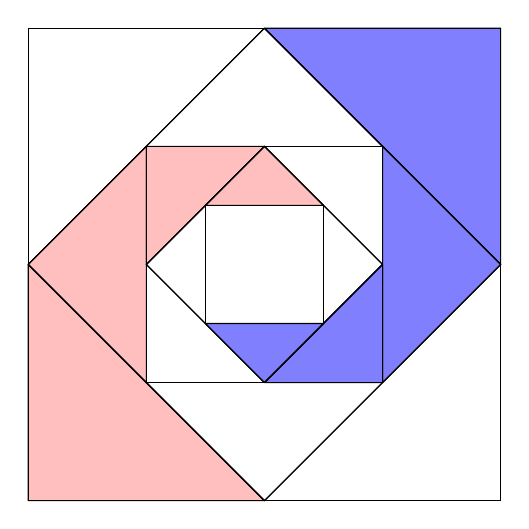
\begin{tikzpicture}[line cap=round,line join=round]
		\def\a{3} % nửa cạnh hình vuông lớn
		\pgfmathsetmacro{\r}{sqrt(2)} % hệ số co của mỗi lần lặp
		%\def{\r}{sqrt(2)} >>> báo lỗi
		%\foreach \i in {0}
		%\fillleftbelow{pink}{\a/pow(sqrt(2),i)}{-45*\i};
		\fillleftbelow{pink}{\a}{0};
		\def\b{\a/1.4142}
		\fillleftbelow{pink}{\b}{-45};
		\def\c{\b/1.4142}
		\fillleftbelow{pink}{\c}{-90};
		\def\d{\c/1.4142}
		\fillleftbelow{pink}{\d}{-135};
		\fillrightabove{blue!50}{\a}{0};
		\fillrightabove{blue!50}{\b}{-45};
		\fillrightabove{blue!50}{\c}{-90};
		\fillrightabove{blue!50}{\d}{-135};
		\draw (A)--(D) (B)--(C);
	\end{tikzpicture}
\end{document}